\renewcommand{\thesection}{\Alph{section}}
\section{Overview}\label{sec:overview}
S\&C will be developed as a multi-tiered, client-server architecture, as shown in Figure \ref{fig:tiers_architecture}. The system will be divided into 
three main layers: the presentation layer, the application layer, and the data layer. The presentation layer will be responsible for managing the user 
interface and the user interaction. The application layer will be responsible for managing the application logic. The data layer will be responsible for 
managing the data storage and the data access.

\begin{figure}[H]
    \centering
    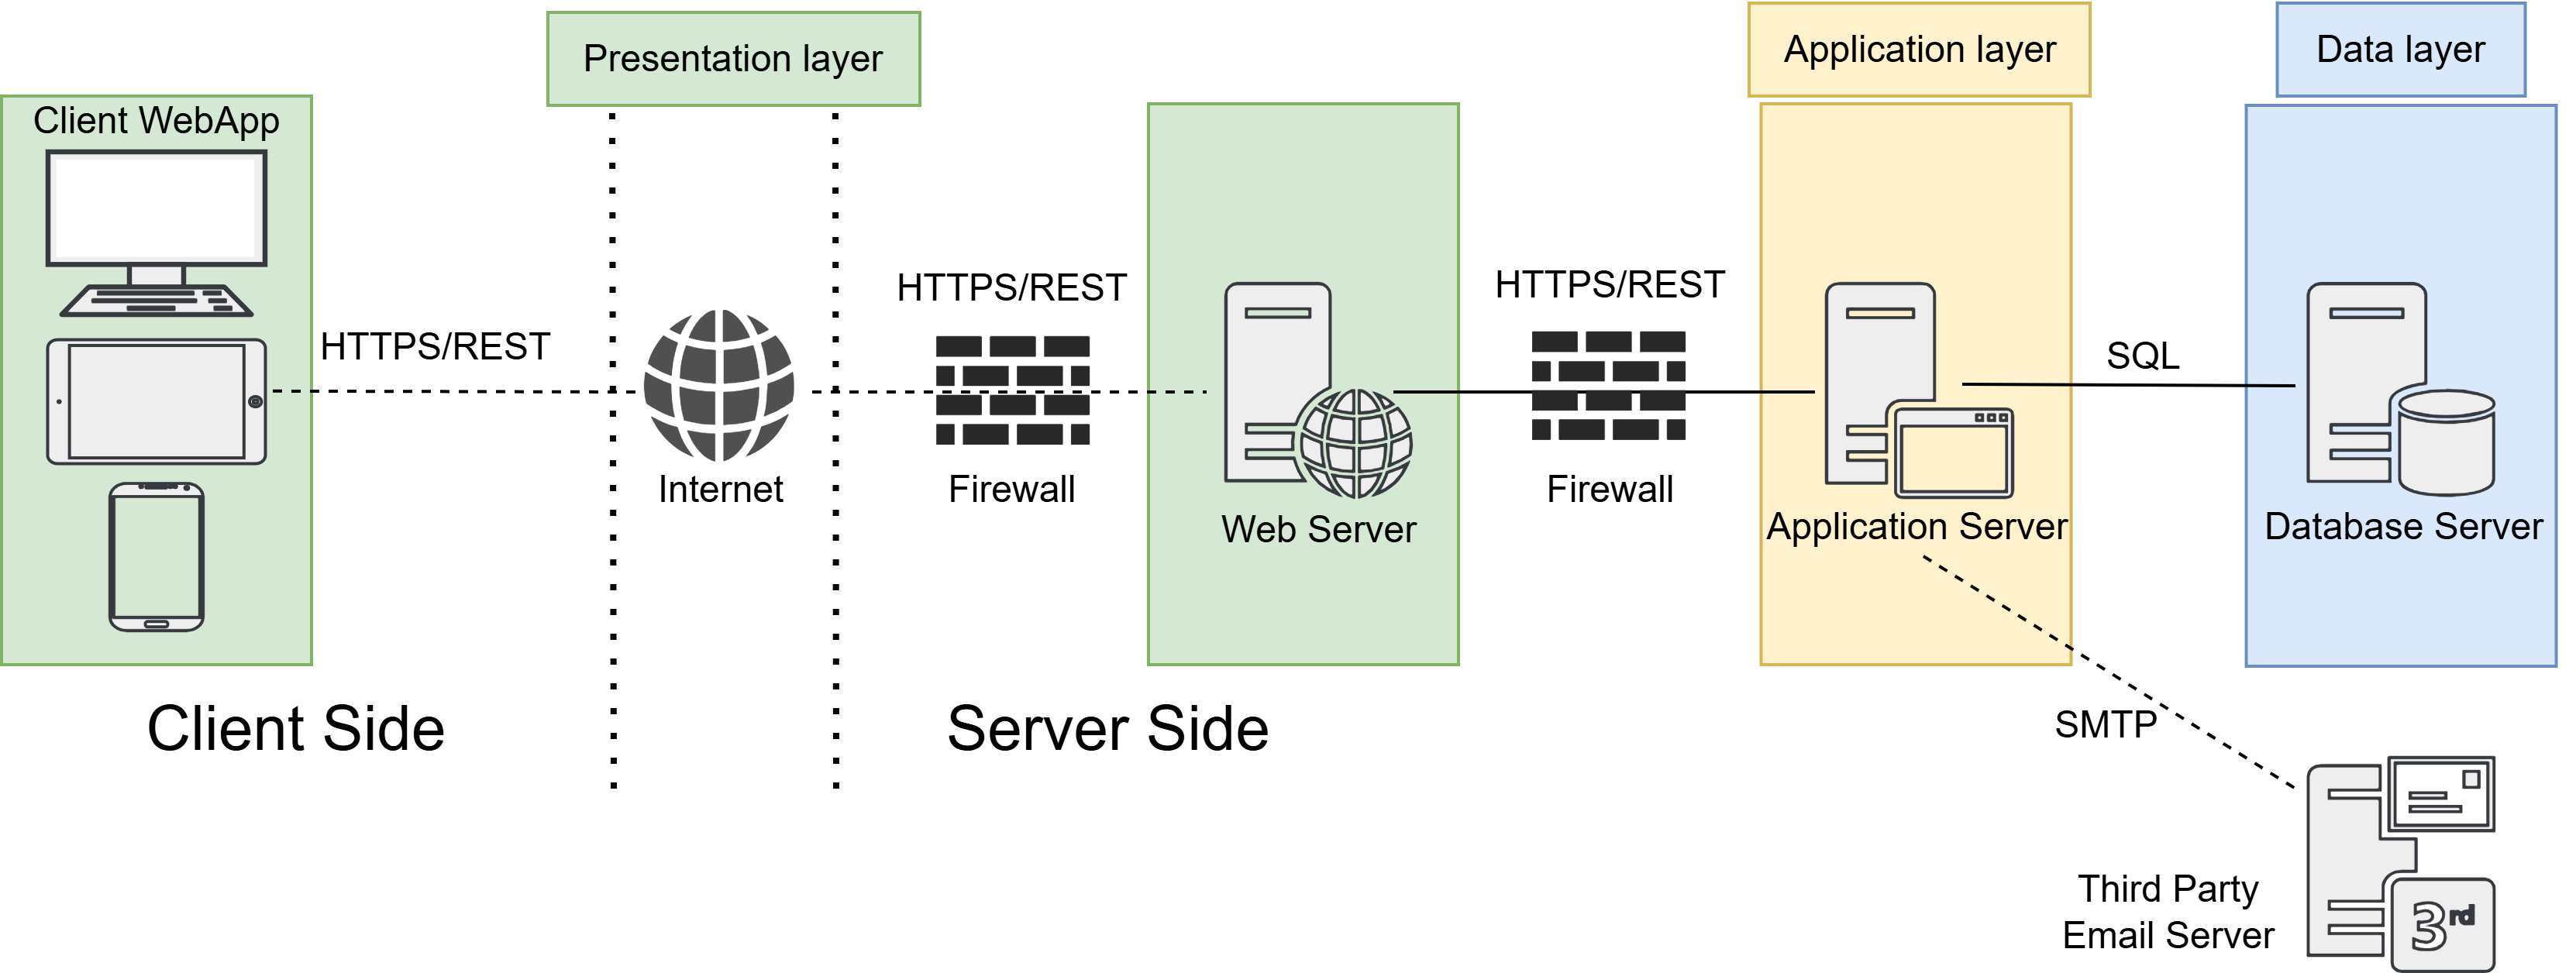
\includegraphics[width=1\textwidth]{Images/tiers_architecture.png}
    \caption{S\&C architectural overview}\label{fig:tiers_architecture}
\end{figure}

In the following paragraph we describe each tier presented in Figure \ref{fig:tiers_architecture}: and what layer it deploys:
\paragraph{Client Side}
\begin{itemize}
    \item \textbf{Web App:} It is the user interface. It will be responsible for managing the user interaction. This means that it will be responsible 
    for hosting part of the presentation layer. 
\end{itemize}

\paragraph{Server Side}
\begin{itemize}
    \item \textbf{Firewall:} It will be responsible for managing the security of the system, by filtering the incoming and outgoing traffic and restricting
    the access based on predefined rules. It will be placed between the Web Server and the Internet and between the Application Server and the Web Server.
    In this way, the web server will reside in a DMZ (Demilitarized Zone), while the application server will resides in a protected internal network.
    \item \textbf{Web Server:} It serves as a gateway between the client and the application server (backend). It will be responsible for hosting part 
    of the presentation layer. For example, it will be responsible for serving the web pages to the client, handling requests routing to the application
    server, managing load balancing, and handling security.
    \item \textbf{Application Server:} It will be responsible for managing the application logic. This means that it will host the application layer. For 
    example, it will be responsible for processing the client requests, execute the business logic, and coordinates with the database and email server.
    \item \textbf{Database Server:} It will be responsible for managing the data storage and the data access. This means that it will host the data layer.
    For example, it will be responsible for storing and retrieving the application data, and executing the database queries.
    \item \textbf{Mail Server:} It will be responsible for managing the email communication. This means that it will be responsible for sending emails to 
    the users. It is triggered by the application server.
\end{itemize}

The Figure\ref{fig:tiers_architecture} also shows how the tiers interact with each other. The Web App interacts with the Web Server through HTTPS/REST 
requests; the Web Server interacts with the Application Server through HTTPS/REST calls; the Application Server interacts with the Database Server through 
SQL queries; and the Application Server interacts with the Mail Server through SMTP requests.

\section{Components view}\label{sec:components view}
\subsection{High-level components and interactions}\label{subsec:high-level components and interactions}
\subsection{Low-level components and interactions}\label{subsec:low-level components and interactions}

\section{Deployment view}\label{sec:deployment view}
\begin{figure}
    \centering
    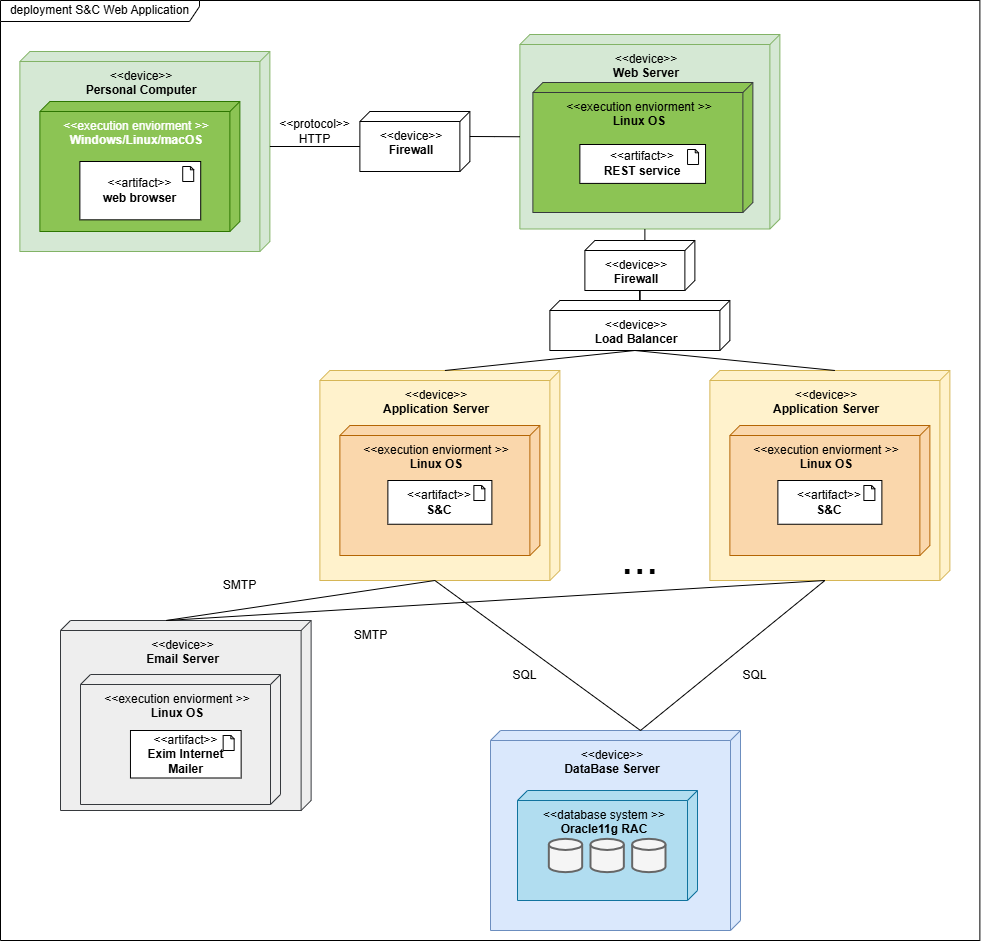
\includegraphics[width=1\textwidth]{Images/DeploymentView.drawio.png}
    \caption{S\&C deployment diagram}\label{fig:deployment_diagram}
\end{figure}
The infrastructure of the S\&C platform is described in below using a deployment diagram and a description of the components and their interactions.
As described at the beginning of this document, the system is divided into three tiers: the presentation layer, the application layer, and the data layer.
The deployment diagram in Figure \ref{fig:deployment_diagram} shows the physical distribution of the components across different servers and the communication
between them.

\begin{itemize}
    \item \textbf{Personal Computer:} Anyone interested in using the platform can access it through any type of personal computer. Users can also access the platform 
    using any device capable of running a web browser. This component communicates and interacts with the Web Server via HTTPS protocols and RESTful API services.
    \item \textbf{Web Server:} The Web Server hosts the web application and serves web pages to users. It handles HTTP requests from clients and forwards them to the 
    Application Server. Together with the Firewall and Load Balancer, it ensures the security, scalability, and availability of the system. It acts as a gateway between
     the client and the Application Server.
    \item \textbf{Application Server:} This component contains the core application logic of the platform, managing the operations necessary to provide services and 
    functionalities to users. Thanks to RESTful API services and the Load Balancer, it can handle multiple requests simultaneously without the risk of overloading or 
    crashing. It interacts with the Database Server to access or store data, such as recording a student's new internship. Additionally, it communicates with the Mail
     Server, particularly during user registration, to authenticate email addresses and verify user identities.
    \item \textbf{Database Server:} Most primary operations of the platform require frequent interaction with the Database Server. This component manages personal data, 
    tracks the progress of applications and internships, stores chat histories between users, and more. The Application Server retrieves or stores data using SQL queries.
    \item \textbf{Mail Server:} During the registration process, the platform requires users to verify their email addresses to confirm their identity and complete 
    account creation. The Application Server interacts with the Mail Server via SMTP requests to send verification emails.
    \item \textbf{Firewall:} The Firewall protects the core components of the system by filtering incoming and outgoing traffic and restricting access based on 
    predefined rules. For example, if an unauthorized individual attempts to access the Application Server and modify data in the Database Server without proper 
    credentials, the Firewall blocks the attempt, preventing unauthorized access.
    \item \textbf{Load Balancer:} The Load Balancer distributes incoming client requests to ensure that no one application server is overwhelmed to operate at peak
        efficiency. It is placed between the Web Server and the Application Server, in order to optimize the performance and availability of the system.
\end{itemize}

\section{Component interfaces}\label{sec:component interfaces}


\section{Runtime view}\label{sec:runtime view}


\section{Selected architectural styles and patterns}\label{sec:selected architectural styles and patterns}
\subsection{Three-Tiered Architecture}\label{subsec:three-tiered architecture}
As described in Section Overview, the Students\&Companies (S\&C) platform is build using a multi-tier architecture. This decision was made with the aim of 
providing a more scalable and flexible system.
The system is divided into three main layers: the presentation layer, the application layer, and the data layer.
Each layer has its own responsibilities and plays a specific role in the system: the presentation layer serves as the front end, accessible through the GUI, 
while the application layer and data layer together form the back end of the system, accessible via API-based methods.
\begin{itemize}
    \item \textbf{Presentation Layer:} The presentation layer is implemented as a generic web application accessible through a web browser.
    It is responsible for managing the presentation logic, including user interaction, the user interface, and rendering information.
    This layer serves as the front end of the system, the only part that the user can access directly.
    \item \textbf{Application Layer:} The application layer is implemented as a set of RESTful web services.
    It is responsible for managing the functional logic of the system, controlling communication between the presentation layer and the data layer.
    This layer allows the system to react to user input and generate appropriate responses accordingly.
    It includes the Application Server and is also used to interact with third-party services.
    \item \textbf{Data Layer:} The data layer is responsible for managing the data storage and access within the system.
    All operations that require data manipulation must be performed through interactions with the data layer.
    The platform uses a Relational Database Management System (RDBMS), making the data accessible through SQL queries.
\end{itemize}
\subsection{RESTful API}\label{subsec:restful api}
The Representational State Transfer (REST) style is designed to be stateless, enabling more efficient and seamless communication between the client and the server.
It uses standard HTTP methods (GET, POST, PUT, DELETE) to perform operations on resources.
The decision to incorporate RESTful APIs into the architecture provides advantages in terms of performance, modifiability, and simplicity by defining conventions 
for interacting with resources in resource-oriented manner.
\subsection{Model-View-Controller (MVC) Pattern}\label{subsec:model-view-controller pattern}
One of the most recommended design patterns for the Three-Tier Architecture is the Model-View-Controller (MVC) pattern. It separates the application into three 
components: the model, the view, and the controller, minimizing interdependencies between the components and improving the maintainability, manageability, and 
scalability of the system. Each component can be developed, tested, and maintained independently.
\begin{itemize}
\item \textbf{Model:} Contains the state and application logic and is independent of the other components.
\item \textbf{View:} Represents the visual presentation logic of the Model and is responsible for displaying data to the user.
\item \textbf{Controller:} Acts as an intermediary between the Model and the View. It receives user input forwarded by the View, then processes operations and 
updates the Model and the View accordingly.
\end{itemize}

\section{Other design decisions}\label{sec:other design decisions}
\begin{itemize}
    \item \textbf{Design patterns related to the behavioral aspects:} Observer Pattern and State Pattern.
    \item \textbf{Design decisions related to the system's requirements:} Some design decisions are already described in the RASD, such as reliability, availability, scalability, security, maintainability, and portability. 
    The following sections revisit availability, scalability, and security to emphasize their importance in the system.
\end{itemize}
\subsection{Observer Pattern}\label{subsec:observer pattern}
The Observer pattern is particularly useful when multiple objects need to be notified about a change in the state of another object. In the context of the S\&C platform, 
a large number of functionalities require the participation of multiple objects, such as notifying users about the results of an interview or updates on the status of an application.
\subsection{State Pattern}\label{subsec:state pattern}
The State pattern is recommended to efficiently manage operations across different states and handle transitions between them, as it allows objects to change their behavior 
when their internal state changes. In the context of the S\&C platform, the State pattern can be used to manage the lifecycle of an application for a internship position.

\subsection{Availability}\label{subsec:availability}
The system is designed to be highly available, ensuring that users can access the platform at any time, as described in the RASD, with at least 99.8 percent uptime. 
To achieve this, critical components should be replicated across multiple servers to provide redundancy and fault tolerance in case of failure. Load balancing is 
correctly configured to distribute incoming traffic, preventing overload on any single server. Continuous monitoring of the system's performance allows for the 
detection and resolution of any issues that may arise in real-time.
\subsection{Scalability}\label{subsec:scalability}
The platform is designed to handle increased user loads in the future by scaling individual layers independently, thanks to the architectural styles and patterns 
mentioned earlier. As described in the RASD, the system can be scaled horizontally by adding more servers or vertically by increasing the resources of existing 
servers, without affecting performance. This scalability is essential, especially as the number of users grows, leading to a higher volume of application requests 
over time.
\subsection{Security}\label{subsec:security}
The system is designed to ensure the privacy and security of user data both during transmission over the network and while stored in the database. This includes the 
use of authentication and authorization mechanisms to ensure that only authorized users can access the system, reducing the risk of unauthorized access. Additionally, 
a firewall and Intrusion Detection System (IDS) are set up in the network to protect the system from external threats and attacks. Protocols like HTTPS are used to 
encrypt communication between the client and server, and other encryption algorithms are employed to protect sensitive data stored in the database, such as user 
passwords.

